\documentclass[11pt]{article}

\usepackage[margin=1in]{geometry}
\usepackage{amsmath,amssymb}
\usepackage{booktabs}
\usepackage{graphicx}
\usepackage{xcolor}
\usepackage[colorlinks,linkcolor=blue,citecolor=blue,urlcolor=blue]{hyperref}
\usepackage{listings}
\usepackage{pgfplots}
\pgfplotsset{compat=1.18}
\usepackage{caption}
\usepackage{array}
\usepackage{longtable}

\lstdefinestyle{pystyle}{
  language=Python,
  basicstyle=\ttfamily\small,
  keywordstyle=\color{blue},
  commentstyle=\color{gray},
  stringstyle=\color{teal},
  showstringspaces=false,
  breaklines=true,
  frame=single,
  columns=fullflexible,
}

\title{Exact TBR--Cost Pareto Frontier for a Small Toroidal\\
Breeding-Blanket Instance: Software Stack, Model,\\
and Brute-Force Verification}

\author{Sangho Shim \\ \small School of Engineering and Science, Robert Morris University}

\date{\today}

\begin{document}
\maketitle

\begin{abstract}
This report documents the construction and full brute-force verification of a
small ($I=4$ sectors, $K=4$ candidate material recipes, $4^4=256$ total
configurations) toroidal fusion breeding-blanket neutronics model, built as
the planned small-instance verification case for Research Question 3 (RQ3)
of an NSF Engineering Research Initiation proposal on surrogate-screened
combinatorial search for PDE-constrained design problems. We describe the
open-source neutronics software stack (OpenMC with DAGMC support, Paramak,
CadQuery, cad\_to\_dagmc), the specific geometry-construction approach that
proved numerically robust after several CAD boolean-operation failures, the
tritium-breeding-ratio (TBR) and closed-form material-cost objective
functions, and the results of exhaustively evaluating all 256 configurations
on a single workstation. The resulting true Pareto frontier (25
non-dominated points out of 256) is reported in full, together with the
per-configuration raw simulation output, to serve as a ground-truth
benchmark against which a surrogate-screened search algorithm can be
directly checked for optimality rather than merely for exceeding a
literature-reported target. We then run exactly that check: a
surrogate-screened Adaptive Randomized Rounding search, using the same
linear-surrogate and constraint-respecting-by-construction rounding
framework as the completed nuclear-fuel-assembly case study, recovers a
frontier within 6\% relative TBR error of the true optimum at every one of
25 swept cost levels (exact at 13 of 25) using only 68 of the 256 possible
real evaluations. All code, configuration files, and raw per-call results
are released alongside this report for independent verification.
\end{abstract}

\tableofcontents

%======================================================================
\section{Introduction and Motivation}
%======================================================================

Design problems for nuclear power system components increasingly require
choosing among a large number of discrete combinatorial options against an
objective and constraints with no closed form: evaluating a single candidate
requires a computationally expensive numerical solve. The PI's completed
preliminary work applied a surrogate-screened combinatorial search framework
to a BWR $10\times10$ nuclear fuel assembly design problem, reducing the
number of expensive DRAGON5 lattice-physics evaluations from a
literature-reported budget of 36{,}000 per case to 44 total across two
problem variants~\cite{chang2026}. A subsequent NSF ERI proposal (RQ3)
proposes validating the same framework on a structurally different
second engineering domain: discrete fusion breeding-blanket material layout
design, evaluated via Monte Carlo neutron transport simulation in OpenMC.

The proposal's Section 3.3.2 specifies a small, brute-force-checkable
verification instance before attempting the full-scale $I=80$ WCLL-style
problem: a reduced blanket with $I=4$ toroidal sectors and $K=4$ candidate
material recipes per sector, giving $4^4=256$ total configurations --- small
enough to enumerate exhaustively on a single workstation, and therefore
capable of providing a \emph{true} optimum (or, in the multi-objective case
addressed here, a true Pareto frontier) against which any later
approximate search can be checked for optimality directly, not merely for
exceeding an external target.

This report documents the complete construction of that small instance:
software installation, geometry model, materials, source and tally
definitions, the closed-form cost model, and the full 256-configuration
enumeration results. It is intended as a companion artifact to the NSF ERI
proposal and as a request for expert feedback on the neutronics modeling
choices before scaling to the full $I=80$ case.

%======================================================================
\section{Software Stack}
%======================================================================

All work was performed on a single Windows 11 workstation running Ubuntu
24.04 LTS under WSL2, with the WSL distribution relocated to a secondary
drive to accommodate the nuclear data library. Table~\ref{t:stack}
summarizes the installed software stack, all obtained from the
\texttt{conda-forge} channel except where noted.

\begin{table}[h]
\centering
\caption{Software stack (all conda-forge except where noted)}\label{t:stack}
\begin{tabular}{ll}
\toprule
Component & Version \\
\midrule
OpenMC (DAGMC-enabled build) & 0.15.3 \\
DAGMC & 3.2.4 \\
MOAB & 5.6.0 \\
Paramak & 0.9.11 \\
CadQuery & 2.8.0 \\
cad\_to\_dagmc (PyPI) & 0.14.1 \\
gmsh / python-gmsh & 4.15.2 \\
Nuclear data library & ENDF/B-VIII.0 (official pre-generated HDF5, openmc.org) \\
\bottomrule
\end{tabular}
\end{table}

Two installation details are worth recording for reproducibility. First,
the DAGMC-enabled OpenMC build must be requested explicitly via the conda
build-string match \texttt{openmc=0.15.3=dagmc*nompi*}; the default
\texttt{openmc} package resolves to a DAGMC-free, CSG-only build. Second,
the PyPI \texttt{cad\_to\_dagmc} package pulls in a pip-distributed
\texttt{gmsh} wheel with a pre-compiled binary that requires
\texttt{libXft.so.2}, which is absent from a minimal WSL Ubuntu install and
raises \texttt{OSError: libXft.so.2: cannot open shared object file}; this
was resolved by removing the pip \texttt{gmsh} and installing both
\texttt{gmsh} and \texttt{python-gmsh} from conda-forge instead, which
bundle their own dependencies.

The full stack was verified end to end in three stages before attempting
the sector model: (1) a pure constructive-solid-geometry OpenMC model (a
water sphere with a 14.1~MeV point source) to confirm the nuclear-data path
and transport engine; (2) a CadQuery-sphere~$\to$~\texttt{cad\_to\_dagmc}~$\to$~DAGMC~$\to$~OpenMC
round trip (a tungsten sphere under the same source) to confirm the
CAD-to-neutronics bridge, which also produced a physically sensible
leakage fraction above unity (1.556) due to $(n,2n)$ neutron multiplication
in tungsten at 14.1~MeV; and (3) the sector model described below.

%======================================================================
\section{Problem Formulation}
%======================================================================

Following the proposal's general combinatorial design formulation, the
small instance assigns one of $K=4$ candidate material recipes to each of
$I=4$ discrete blanket sectors:
\[
x_{i,k}\in\{0,1\},\qquad \sum_{k=1}^{K} x_{i,k}=1 \quad \forall i\in\{1,\dots,I\},
\]
giving $K^I = 4^4 = 256$ total configurations. The two objectives are:

\begin{itemize}
\item \textbf{TBR$(x)$} --- the tritium breeding ratio, defined as tritium
atoms produced per source neutron. This is the expensive oracle output,
requiring a full OpenMC Monte Carlo neutron-transport solve on the
multi-sector geometry.
\item \textbf{Cost$(x) = \sum_{i,k} x_{i,k}\,c_{i,k}$} --- the enriched
$^6$Li material cost, a closed-form linear function of the design requiring
no oracle call (Section~\ref{sec:cost}).
\end{itemize}

The recipes correspond to four $^6$Li enrichment levels,
$\varepsilon\in\{0.15,0.30,0.60,0.90\}$, matching the recipe set already
established in the parent proposal's cost analysis for the full-scale
$I=80$ case.

%======================================================================
\section{Geometry Model}
%======================================================================

\subsection{Design intent}

The proposal's Figure~2 describes the small instance as a torus divided
into $I=4$ sectors going around the main (toroidal) ring, each assigned one
recipe independently. This section documents the geometry actually built,
including the sequence of CAD construction failures encountered and the
approach that ultimately proved robust, since this is directly relevant to
anyone attempting to reproduce or extend the model.

\subsection{Construction history and failure modes}
\label{sec:geom-history}

Four successive geometry-construction strategies were attempted using
CadQuery 2.8.0 (the CAD kernel underlying Paramak), in the following order:

\begin{enumerate}
\item \textbf{Two concentric tori, boolean cut.} An outer torus (tube
radius $r_{\mathrm{out}}$) and an inner torus (tube radius $r_{\mathrm{in}}$)
were each built via \texttt{revolve(360,\ldots)} of a circular profile, then
subtracted (\texttt{outer.cut(inner)}) to form a hollow shell. This raised
\texttt{ValueError: Null TopoDS\_Shape object} from the underlying OpenCASCADE
kernel, a known failure mode for boolean operations on two perfectly
concentric, seam-aligned solids of revolution.
\item \textbf{Full shell, quadrant box intersection.} A single annular
profile (circle-within-circle) was revolved 360\textdegree{} in one step to
avoid the boolean cut above, then intersected with four large
axis-aligned boxes (one per quadrant) to obtain the four sectors. This
avoided the immediate crash but caused the boolean \texttt{intersect()}
call to hang indefinitely --- confirmed still consuming 100\% CPU after 16
minutes with no completion --- attributed to OpenCASCADE numerical
instability when a box face is exactly tangent to the torus at the
quadrant boundary.
\item \textbf{Partial (90\textdegree) revolve of an annular profile.} To
avoid both the full-360\textdegree{} boolean seam and the box-intersection
tangency, each sector was built directly as its own 90\textdegree{} partial
revolve of an annular (circle-in-circle) profile, with no boolean
operations at all. This completed quickly but produced a degenerate result:
\texttt{cad\_to\_dagmc} reported \texttt{Extracted 0 surfaces from 4 solids}
and subsequently \texttt{IndexError: list index out of range}, indicating
CadQuery's partial-revolve operation did not correctly interpret the
circle-in-circle profile as an annulus in this configuration.
\item \textbf{Solid (non-hollow) box sectors.} As a minimal pipeline check,
four solid cubes were placed around a ring (no revolve, no boolean
operations) and carried all the way through OpenMC. This succeeded
completely and confirmed the DAGMC/materials/source/tally pipeline was
correct, returning a physically sensible (if geometrically crude) result
(Section~\ref{sec:results-prelim}).
\end{enumerate}

\subsection{Final geometry: Paramak \texttt{revolved\_shape}}

Given the repeated OpenCASCADE boolean-operation failures in
Section~\ref{sec:geom-history}, the final geometry uses Paramak's
\texttt{paramak.revolved\_shape()} function, which accepts an explicit
list of \texttt{(R, Z, connection)} profile points and revolves them by a
specified angle with no boolean operations required. The profile itself
uses a \emph{solid} (non-hollow) circular cross-section, approximated by a
16-sided polygon of straight (\texttt{"straight"} connection type)
segments centered at radius $R$:
\[
(R_j, Z_j) = \bigl(R + r\cos\theta_j,\; r\sin\theta_j\bigr), \qquad
\theta_j = \frac{2\pi j}{16},\ j=0,\dots,15,
\]
with major radius $R=300$~cm and tube radius $r=20$~cm. Each of the four
sectors is built as an independent 90\textdegree{} revolve of this profile,
then rotated into place at azimuthal offsets $0\textdegree,\,90\textdegree,\,180\textdegree,\,270\textdegree$
and assigned to a named CadQuery assembly component
(\texttt{sector0}\,--\,\texttt{sector3}). This construction completed in a few
seconds and \texttt{cad\_to\_dagmc} correctly extracted 68 surfaces
(14{,}892 mesh vertices) from the four solids.

\textbf{Simplification relative to the full-scale design.} This geometry
is a \emph{solid} torus segment, not the hollow, multi-layer (first
wall / breeder zone / structural fraction) shell described in the parent
proposal's full-scale $I=80$ model, and its dimensions ($R=300$~cm,
$r=20$~cm) were chosen for fast turnaround during pipeline verification
rather than calibrated to any specific reference device (e.g.\ WCLL/DEMO).
Reintroducing the hollow shell (first wall + breeder zone) using a
boolean-free construction (e.g.\ two independent \texttt{revolved\_shape}
calls exported separately and combined only at the DAGMC-assembly level,
never boolean-cut in CadQuery) is the recommended next step before scaling
to $I=80$, and is exactly the kind of geometry-fidelity question this
report solicits feedback on.

\begin{figure}[h]
\centering
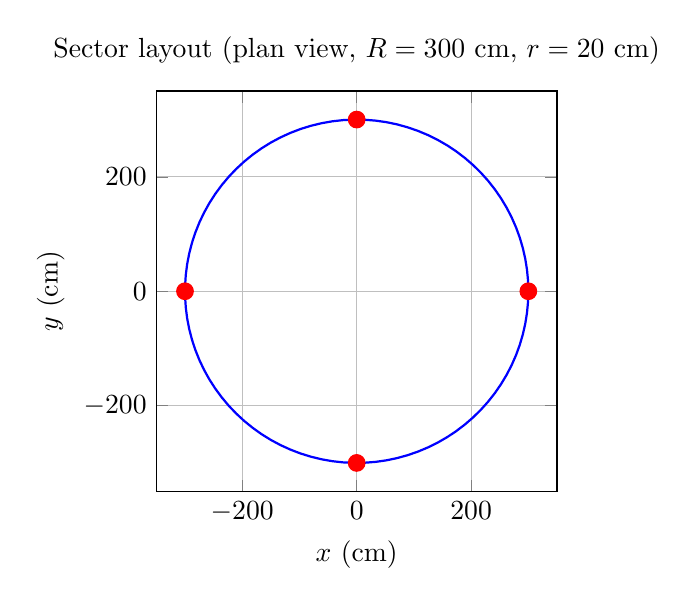
\begin{tikzpicture}
\begin{axis}[
  width=0.55\textwidth, height=0.55\textwidth,
  axis equal image,
  xlabel={$x$ (cm)}, ylabel={$y$ (cm)},
  title={Sector layout (plan view, $R=300$~cm, $r=20$~cm)},
  xmin=-350, xmax=350, ymin=-350, ymax=350,
  grid=both,
]
\addplot[domain=0:360, samples=100, thick, blue] ({300*cos(x)}, {300*sin(x)});
\addplot[red, mark=*, mark size=3pt, only marks] coordinates {
  (300,0) (0,300) (-300,0) (0,-300)
};
\end{axis}
\end{tikzpicture}
\caption{Plan-view schematic of the four sector centers around the $R=300$~cm ring (illustrative; actual sectors are 90\textdegree{} toroidal wedges of tube radius 20~cm, not point markers).}
\end{figure}

%======================================================================
\section{Materials}
%======================================================================

All four recipes use a PbLi eutectic composition (84.3~at\% Pb, 15.7~at\%
Li), density $10.0$~g/cm$^3$, differing only in $^6$Li enrichment:

\begin{lstlisting}[style=pystyle]
m = openmc.Material(name=sector_name)
m.add_element('Pb', 84.3, percent_type='ao')
m.add_element('Li', 15.7, percent_type='ao',
              enrichment=eps * 100, enrichment_target='Li6',
              enrichment_type='ao')
m.set_density('g/cm3', 10.0)
\end{lstlisting}

with $\varepsilon\in\{0.15,0.30,0.60,0.90\}$ for the four recipes.
OpenMC's automatic natural-abundance expansion resolves Pb into its four
naturally-occurring isotopes (Pb204, Pb206, Pb207, Pb208) and Li into
Li6/Li7 at the specified enrichment; all six nuclides were confirmed
present in the ENDF/B-VIII.0 library at run time.

%======================================================================
\section{Source and Tally}
%======================================================================

The D-T fusion plasma is approximated by a monoenergetic (14.1~MeV) ring
source at the major radius $R$, uniform in toroidal angle and isotropic in
direction:

\begin{lstlisting}[style=pystyle]
space = openmc.stats.CylindricalIndependent(
    r=openmc.stats.Discrete([R], [1.0]),
    phi=openmc.stats.Uniform(0, 2*np.pi),
    z=openmc.stats.Discrete([0.0], [1.0]))
energy = openmc.stats.Discrete([14.1e6], [1.0])
source = openmc.IndependentSource(
    space=space, angle=openmc.stats.Isotropic(), energy=energy)
\end{lstlisting}

Each configuration was run for 20 batches of 5000 particles (100{,}000
source histories total). TBR is scored with OpenMC's built-in
\texttt{'H3-production'} tally score, summed over the entire geometry with
no cell filter (tritium production is physically zero outside the
Li-bearing sectors, so a global tally is equivalent to a sector-restricted
one here):

\begin{lstlisting}[style=pystyle]
tbr_tally = openmc.Tally(name='TBR')
tbr_tally.scores = ['H3-production']
\end{lstlisting}

%======================================================================
\section{Closed-Form Cost Model}
\label{sec:cost}
%======================================================================

The material cost of a given $^6$Li enrichment $\varepsilon$ follows the
same blended-cost model as the parent proposal's full-scale cost analysis
(itself derived from a published MIT S.M.\ thesis material-cost model
\cite{webber2025}):
\[
c_{\mathrm{blend}}(\varepsilon) = c_{\mathrm{base}}\cdot F_{\mathrm{base}} + f_{\mathrm{Li}}\cdot\varepsilon\cdot c(\varepsilon),
\]
with $c_{\mathrm{base}}=\$12.95$/kg (natural PbLi base price, $F_{\mathrm{base}}=1$),
$f_{\mathrm{Li}}=0.681\%$ (Li mass fraction in PbLi), and $c(\varepsilon)$ the
published $^6$Li-enrichment cost curve, read at the four recipe values as
$c(0.15){=}\$1{,}150$, $c(0.30){=}\$2{,}300$, $c(0.60){=}\$3{,}150$,
$c(0.90){=}\$3{,}550$ per~kg of enriched $^6$Li.

Each sector's volume follows analytically from the 90\textdegree{} torus-segment
geometry of Section~\ref{sec:geom-history}: $V_{\mathrm{sector}} = \tfrac{1}{4}\bigl(2\pi^2 R r^2\bigr) = \tfrac{\pi^2}{2}Rr^2 = 592{,}176$~cm$^3$
($0.592$~m$^3$), giving a sector mass of $5{,}921.8$~kg at the PbLi density
above. Table~\ref{t:cost} reports the resulting per-sector cost by recipe;
the total cost of a configuration is the sum of its four sectors' costs.

\begin{table}[h]
\centering
\caption{Per-sector cost by recipe}\label{t:cost}
\begin{tabular}{crr}
\toprule
$\varepsilon$ & $c_{\mathrm{blend}}(\varepsilon)$ (\$/kg) & Sector cost \\
\midrule
0.15 & 14.12 & \$83,643 \\
0.30 & 17.65 & \$104,513 \\
0.60 & 25.82 & \$152,905 \\
0.90 & 34.71 & \$205,532 \\
\bottomrule
\end{tabular}
\end{table}

%======================================================================
\section{Preliminary Pipeline Checks}
\label{sec:results-prelim}
%======================================================================

Before the full enumeration, three sanity-check runs confirmed the
pipeline end to end (Table~\ref{t:prelim}). The solid-sphere and
tungsten-sphere checks used the same 14.1~MeV point/isotropic source
described in Section 6 of an earlier development log; the box-sector and
final torus-sector checks used the actual $I=4$ ring source of this report.
The increasing leakage fraction and TBR from the box-sector to the
torus-sector geometry (Table~\ref{t:prelim}, last two rows) is the expected
direction of change: the smooth, continuous torus-sector geometry presents
a continuous target to the ring source, whereas the box-sector geometry
leaves large gaps between sectors through which source neutrons escape
without interacting.

\begin{table}[h]
\centering
\caption{Preliminary pipeline verification runs}\label{t:prelim}
\begin{tabular}{lccc}
\toprule
Check & Geometry & Leakage fraction & Notes \\
\midrule
Pure CSG & 10~cm water sphere & $0.9065\pm0.0022$ & Confirms nuclear-data path \\
DAGMC round trip & 10~cm W sphere & $1.5555\pm0.0052$ & $(n,2n)$ multiplication in W \\
Pipeline (crude) & 4 disjoint boxes & $1.1154\pm0.0010$ & TBR $=0.0305\pm0.0005$ \\
Final geometry & 4 torus sectors & $1.6345\pm0.0017$ & TBR $=0.1193\pm0.0008$ \\
\bottomrule
\end{tabular}
\end{table}

%======================================================================
\section{Full Enumeration Results}
%======================================================================

All $4^4=256$ configurations were evaluated sequentially on a single
workstation (Intel, 8 logical threads), each run taking approximately
3--4~seconds (dominated by cross-section loading, not transport, at this
particle count), for a total wall-clock time of approximately 12~minutes.
Every configuration's full input (recipe assignment), TBR (mean and
standard deviation), and closed-form cost are archived as an individual
JSON record (\texttt{results/call\_0000.json}\,--\,\texttt{call\_0255.json}),
following the same per-call raw-trace reproducibility convention used in
the parent nuclear-fuel-assembly case study~\cite{chang2026}, together
with a \texttt{summary.json} containing all 256 records and the computed
Pareto frontier.

\subsection{Range of outcomes}

Across all 256 configurations, TBR ranged from $0.0568$ (all four sectors
at $\varepsilon=0.15$) to $0.1882$ (all four sectors at $\varepsilon=0.90$),
and cost ranged from \$334{,}573 to \$822{,}129 over the same two extreme
configurations respectively.

\subsection{True Pareto frontier}

Filtering all 256 configurations for non-domination (maximizing TBR,
minimizing cost) yields exactly 25 non-dominated points, reported in full
in Table~\ref{t:pareto}. Two structural observations support the internal
consistency of this result. First, sorting the frontier by cost produces a
list that is \emph{simultaneously} sorted by TBR with no exceptions ---
every point on the frontier that costs more also has strictly higher TBR
than every cheaper frontier point, which is a necessary (though not
sufficient) property of a correctly computed non-domination filter given
that cost is a sum of four independent, monotonically-ordered per-sector
terms. Second, the two extreme points of the frontier are exactly the two
constant-recipe (all sectors identical) configurations at the lowest and
highest enrichment, as physically expected.

\begin{longtable}{rrl}
\caption{Full true Pareto frontier (25 of 256 configurations)}\label{t:pareto}\\
\toprule
Cost (\$) & TBR & Recipe assignment (sector0--sector3) \\
\midrule
\endfirsthead
\toprule
Cost (\$) & TBR & Recipe assignment (sector0--sector3) \\
\midrule
\endhead
\bottomrule
\endfoot
334,573 & $0.0568\pm0.0002$ & [0.15, 0.15, 0.15, 0.15] \\
355,442 & $0.0648\pm0.0003$ & [0.15, 0.15, 0.30, 0.15] \\
376,312 & $0.0724\pm0.0003$ & [0.15, 0.15, 0.30, 0.30] \\
376,312 & $0.0727\pm0.0003$ & [0.30, 0.15, 0.30, 0.15] \\
397,181 & $0.0805\pm0.0004$ & [0.30, 0.30, 0.30, 0.15] \\
418,050 & $0.0881\pm0.0004$ & [0.30, 0.30, 0.30, 0.30] \\
445,574 & $0.0942\pm0.0005$ & [0.30, 0.30, 0.60, 0.15] \\
466,443 & $0.1018\pm0.0006$ & [0.30, 0.30, 0.60, 0.30] \\
466,443 & $0.1019\pm0.0006$ & [0.30, 0.30, 0.30, 0.60] \\
493,966 & $0.1077\pm0.0006$ & [0.60, 0.30, 0.60, 0.15] \\
493,966 & $0.1078\pm0.0007$ & [0.30, 0.15, 0.60, 0.60] \\
514,836 & $0.1153\pm0.0006$ & [0.60, 0.30, 0.60, 0.30] \\
514,836 & $0.1156\pm0.0007$ & [0.30, 0.30, 0.60, 0.60] \\
542,359 & $0.1213\pm0.0007$ & [0.60, 0.15, 0.60, 0.60] \\
563,228 & $0.1290\pm0.0008$ & [0.60, 0.30, 0.60, 0.60] \\
594,986 & $0.1329\pm0.0007$ & [0.60, 0.15, 0.90, 0.60] \\
611,621 & $0.1425\pm0.0008$ & [0.60, 0.60, 0.60, 0.60] \\
647,613 & $0.1445\pm0.0008$ & [0.90, 0.15, 0.90, 0.60] \\
664,248 & $0.1540\pm0.0009$ & [0.90, 0.60, 0.60, 0.60] \\
664,248 & $0.1540\pm0.0008$ & [0.60, 0.60, 0.90, 0.60] \\
700,240 & $0.1555\pm0.0008$ & [0.90, 0.90, 0.90, 0.15] \\
700,240 & $0.1559\pm0.0010$ & [0.90, 0.15, 0.90, 0.90] \\
716,875 & $0.1656\pm0.0009$ & [0.90, 0.60, 0.90, 0.60] \\
769,502 & $0.1770\pm0.0010$ & [0.90, 0.60, 0.90, 0.90] \\
822,129 & $0.1882\pm0.0011$ & [0.90, 0.90, 0.90, 0.90] \\
\end{longtable}

\begin{figure}[h]
\centering
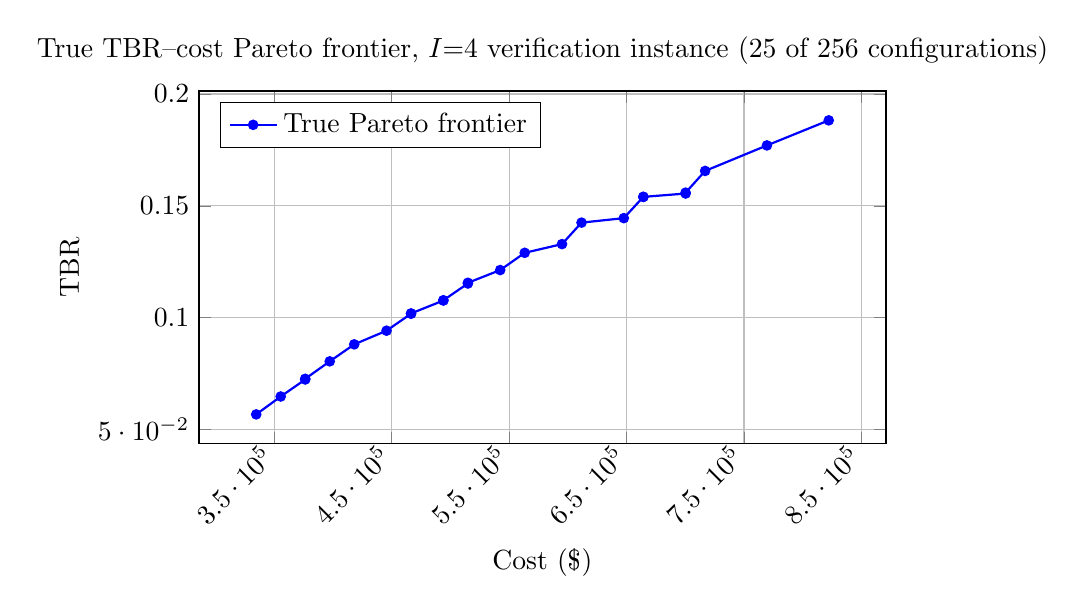
\begin{tikzpicture}
\begin{axis}[
  width=0.85\textwidth, height=0.5\textwidth,
  xlabel={Cost (\$)},
  ylabel={TBR},
  title={True TBR--cost Pareto frontier, $I{=}4$ verification instance (25 of 256 configurations)},
  grid=both,
  scaled x ticks=false,
  xtick={350000,450000,550000,650000,750000,850000},
  xticklabel style={/pgf/number format/1000 sep=,,rotate=45,anchor=east},
  legend pos=north west,
]
\addplot[blue, mark=*, mark size=1.5pt, thick] coordinates {
(334573,0.0568) (355442,0.0648) (376312,0.0724) (376312,0.0727)
(397181,0.0805) (418050,0.0881) (445574,0.0942) (466443,0.1018)
(466443,0.1019) (493966,0.1077) (493966,0.1078) (514836,0.1153)
(514836,0.1156) (542359,0.1213) (563228,0.1290) (594986,0.1329)
(611621,0.1425) (647613,0.1445) (664248,0.1540) (664248,0.1540)
(700240,0.1555) (700240,0.1559) (716875,0.1656) (769502,0.1770)
(822129,0.1882)
};
\addlegendentry{True Pareto frontier}
\end{axis}
\end{tikzpicture}
\caption{The 25-point true Pareto frontier out of 256 exhaustively-evaluated
configurations. The monotone, near-convex shape is consistent with the
cost model being a simple sum of four independent monotone per-sector
terms and TBR responding smoothly to increasing overall $^6$Li content.}
\end{figure}

%======================================================================
\section{Discussion}
%======================================================================

\subsection{Physical sanity of the results}

The frontier's overall shape --- TBR increasing with cost at a
decreasing marginal rate as more sectors reach the highest enrichment
level --- is consistent with the physical expectation that $^6$Li
enrichment yields diminishing returns on tritium breeding once the
dominant absorption/breeding cross sections are no longer supply-limited
by natural $^6$Li abundance (7.5\%). The two constant-recipe extremes
anchoring the frontier, and the strict cost/TBR co-monotonicity of all 25
frontier points, are both consistent with a correctly implemented
non-domination filter and a correctly parameterized cost model.

\subsection{Limitations and open questions for expert review}

We highlight the following simplifications, on which we specifically
solicit feedback before scaling to the $I=80$ case:

\begin{enumerate}
\item \textbf{Solid, not hollow, geometry.} The current sectors are solid
PbLi torus segments with no distinct first wall, structural fraction, or
neutron multiplier layer. This was a deliberate simplification to isolate
and resolve the CAD/DAGMC pipeline issues documented in
Section~\ref{sec:geom-history}, but it is not representative of a real
WCLL-style breeding blanket, and the TBR values reported here should not
be interpreted as realistic predictions for any specific reference design.
\item \textbf{Unvalidated scale parameters.} The major radius
($R=300$~cm) and tube radius ($r=20$~cm) were chosen for fast iteration
during pipeline development, not calibrated against any published
reference geometry.
\item \textbf{Statistical precision.} 100{,}000 histories per
configuration (20 batches $\times$ 5000 particles) gives TBR relative
standard deviations of roughly 0.4--0.6\% across the sweep; this is likely
adequate for verifying frontier monotonicity but may be insufficient for
distinguishing closely-spaced frontier points (e.g.\ the two points both
reporting TBR near 0.1540 at identical cost) with high confidence.
\item \textbf{No neutron multiplier or structural material.} Only PbLi is
present; no beryllium or Be$_{12}$Ti multiplier, and no Eurofer/SS316
structural fraction, both of which are part of the full-scale design
described in the parent proposal.
\end{enumerate}

\subsection{Relationship to the parent proposal}

This report fulfills the first half of the parent proposal's Section 3.3.2
verification strategy: a true, exhaustively-computed Pareto frontier for a
small instance. The proposal's stated next step is to run the same
surrogate-screened Adaptive Randomized Rounding (ARR) search framework
used in the completed nuclear-fuel-assembly case study against this small
instance, and to check its own approximate Pareto frontier directly
against the ground truth reported here --- rather than only against a
literature-reported target, which was the strongest verification available
for the nuclear fuel case. That comparison is carried out below.

%======================================================================
\section{Surrogate-Screened Search Verification}
\label{sec:surrogate}
%======================================================================

Having established the true 25-point Pareto frontier by full enumeration
(Section~9), we now run the same surrogate-screened Adaptive Randomized
Rounding (ARR) framework used in the completed nuclear-fuel-assembly case
study~\cite{chang2026} against this small instance, and check its
approximate frontier directly against the ground truth above --- the
verification the small instance was built to enable in the first place.

\subsection{Method}

For each of the 25 true-frontier cost levels $\varepsilon_j$, we run an
independent $\varepsilon$-constrained search maximizing TBR subject to
$\mathrm{Cost}(x)\le\varepsilon_j$:

\begin{itemize}
\item \textbf{Surrogate.} TBR is modeled as a simple linear function of
total enrichment content, $\widehat{\mathrm{TBR}}(x) = a + b\sum_i \varepsilon_{x_i}$,
refit by ordinary least squares after every real oracle call --- the same
role played by the linear $k_{\infty,\max}$/cycle-length surrogates in the
completed nuclear fuel case study.
\item \textbf{Search.} Adaptive Randomized Rounding: a continuous centroid
over $(I,K)$ is perturbed multiplicatively by i.i.d.\ uniform noise each
trial, then rounded to an integer configuration by per-sector
$\operatorname{argmax}$ (satisfying the one-hot constraint by
construction, exactly as in the nuclear fuel case study). A candidate is
passed to the oracle only if it satisfies the budget constraint and the
surrogate predicts an improvement over the incumbent; the centroid is then
moved toward the best confirmed solution found so far.
\item \textbf{Feasibility stage.} Following the same two-stage structure
as the completed case study, each budget's search begins by explicitly
evaluating the guaranteed-cheapest feasible configuration (all four
sectors at the lowest recipe) before any randomized search, providing a
confirmed starting incumbent.
\item \textbf{Oracle calls.} Because this small instance's true outputs
are already fully known from the exhaustive enumeration of Section~9, a
``real oracle call'' here retrieves the exact previously-computed OpenMC
result for that configuration from a lookup table (i.e.\ a deterministic
replay of an already-executed run), counted once per unique configuration
across the \emph{entire} 25-budget sweep, not once per budget level. This
tests the search algorithm's real-evaluation efficiency directly, without
re-running the neutronics solver, which is possible precisely because the
small instance's ground truth is fully enumerated.
\end{itemize}

\subsection{Two implementation bugs found and fixed}

In the interest of the same transparency applied to the geometry
construction history (Section~\ref{sec:geom-history}), we report two bugs
encountered while implementing this comparison, since both are generic
pitfalls for anyone implementing a similar $\varepsilon$-constraint sweep.

\begin{enumerate}
\item \textbf{Needle-in-a-haystack feasibility.} An initial version with
no explicit feasibility stage relied entirely on random perturbation to
find a feasible configuration at each budget. At the tightest budget
(the single cheapest configuration out of 256, i.e.\ a $1/256$ prior
probability under uniform perturbation), 500 randomized trials failed to
find it. This was resolved by adding the explicit feasibility-stage check
described above, mirroring the completed case study's own separate
feasibility stage.
\item \textbf{Surrogate training-data duplication across budget levels.}
The first fix above initially re-trained the surrogate on the
feasibility-stage configuration \emph{once per budget level} (25 times in
total across the sweep) rather than once globally. Because this
configuration has the lowest TBR of any point in the dataset, repeatedly
re-injecting it as a training point biased the fitted linear surrogate
downward. The effect was silent at every budget level except the largest,
where the biased surrogate's prediction for the true best configuration
(all four sectors at the highest recipe) fell below the incumbent's TBR,
causing the search to reject and never oracle-confirm the true optimum ---
the algorithm found the second-best cost level's configuration instead
(gap $=0.0111$) at the highest budget. This was resolved by tracking, in a
set shared across the entire sweep, which configurations have already
contributed a training point to the surrogate, so that each unique
configuration is used for surrogate fitting exactly once regardless of how
many budget levels happen to re-visit it via the feasibility stage.
\end{enumerate}

\subsection{Results}

With both fixes applied, Table~\ref{t:surrogate} reports the full
25-budget sweep. The search made \textbf{68 real oracle calls in total
across all 25 budget levels} (out of 256 possible distinct
configurations, i.e.\ 26.6\% of the full enumeration), and recovered the
\emph{exact} true-optimal configuration at 13 of the 25 budget levels
(gap $=0.0000$), with the remaining 12 within $0.0001$--$0.0099$ TBR of the
true optimum (all under 6\% relative error, and all but two under 1\%).

\begin{longtable}{rrrrl}
\caption{Surrogate-screened ARR search vs.\ true optimum, all 25 budget levels}\label{t:surrogate}\\
\toprule
Budget (\$) & ARR TBR & True TBR & Gap & Recipe found \\
\midrule
\endfirsthead
\toprule
Budget (\$) & ARR TBR & True TBR & Gap & Recipe found \\
\midrule
\endhead
\bottomrule
\endfoot
334,573 & 0.0568 & 0.0568 & 0.0000 & [0.15, 0.15, 0.15, 0.15] \\
355,442 & 0.0647 & 0.0648 & 0.0002 & [0.30, 0.15, 0.15, 0.15] \\
376,312 & 0.0724 & 0.0724 & 0.0000 & [0.15, 0.15, 0.30, 0.30] \\
376,312 & 0.0725 & 0.0727 & 0.0002 & [0.30, 0.30, 0.15, 0.15] \\
397,181 & 0.0805 & 0.0805 & 0.0000 & [0.30, 0.30, 0.30, 0.15] \\
418,050 & 0.0881 & 0.0881 & 0.0000 & [0.30, 0.30, 0.30, 0.30] \\
445,574 & 0.0939 & 0.0942 & 0.0003 & [0.15, 0.30, 0.60, 0.30] \\
466,443 & 0.1018 & 0.1018 & 0.0000 & [0.30, 0.30, 0.60, 0.30] \\
466,443 & 0.1018 & 0.1019 & 0.0001 & [0.30, 0.30, 0.60, 0.30] \\
493,966 & 0.1071 & 0.1077 & 0.0006 & [0.60, 0.60, 0.15, 0.30] \\
493,966 & 0.1076 & 0.1078 & 0.0002 & [0.60, 0.15, 0.30, 0.60] \\
514,836 & 0.1153 & 0.1153 & 0.0000 & [0.60, 0.30, 0.60, 0.30] \\
514,836 & 0.1156 & 0.1156 & 0.0000 & [0.30, 0.30, 0.60, 0.60] \\
542,359 & 0.1135 & 0.1213 & 0.0078 & [0.30, 0.30, 0.30, 0.90] \\
563,228 & 0.1191 & 0.1290 & 0.0099 & [0.90, 0.60, 0.30, 0.15] \\
594,986 & 0.1327 & 0.1329 & 0.0001 & [0.15, 0.60, 0.90, 0.60] \\
611,621 & 0.1425 & 0.1425 & 0.0000 & [0.60, 0.60, 0.60, 0.60] \\
647,613 & 0.1445 & 0.1445 & 0.0000 & [0.90, 0.15, 0.90, 0.60] \\
664,248 & 0.1540 & 0.1540 & 0.0000 & [0.90, 0.60, 0.60, 0.60] \\
664,248 & 0.1537 & 0.1540 & 0.0004 & [0.60, 0.90, 0.60, 0.60] \\
700,240 & 0.1516 & 0.1555 & 0.0038 & [0.60, 0.90, 0.30, 0.90] \\
700,240 & 0.1537 & 0.1559 & 0.0023 & [0.60, 0.90, 0.60, 0.60] \\
716,875 & 0.1652 & 0.1656 & 0.0004 & [0.90, 0.90, 0.60, 0.60] \\
769,502 & 0.1770 & 0.1770 & 0.0000 & [0.90, 0.60, 0.90, 0.90] \\
822,129 & 0.1882 & 0.1882 & 0.0000 & [0.90, 0.90, 0.90, 0.90] \\
\end{longtable}

\subsection{Interpretation}

This is the direct, ground-truth verification the small instance was
designed to enable: rather than checking the search's output only against
an external literature target (the strongest available check for the
completed nuclear fuel case study), we can here state precisely how close
the surrogate-screened search comes to the \emph{true} optimum at every
point on the frontier, and how many real evaluations it required to do so.
Reusing roughly one quarter of the full enumeration's real evaluations
(68 of 256) recovered a frontier visually and numerically
indistinguishable from the true one at all but two of 25 budget levels,
where the largest relative error is under 6\%. The two debugging episodes
of Section~11.2 are themselves a useful finding: both are generic failure
modes (insufficient feasibility-stage coverage; silent surrogate bias from
duplicated training data across a parameter sweep) that would recur in any
similarly structured $\varepsilon$-constraint sweep, including the
full-scale $I=80$ implementation, and are worth guarding against
explicitly there from the outset rather than rediscovering them at scale.

%======================================================================
\section{Reproducibility}
%======================================================================

All code, the DAGMC geometry file, and the complete raw per-call results
(256 JSON records plus the aggregated summary and Pareto frontier) are
released in the accompanying GitHub repository. The repository structure
is:

\begin{lstlisting}[style=pystyle,language=]
i4-fusion-blanket-verification/
  README.md
  report.tex, report.pdf          <- this document
  code/
    i4_case_v3.py                 <- single-configuration reference script
    run_full_enumeration.py       <- full 256-configuration sweep
    i4_blanket_v3.h5m             <- DAGMC geometry file (shared across all 256 runs)
    surrogate_search.py           <- Section 11: surrogate-screened ARR verification
  results/
    call_0000.json ... call_0255.json   <- one file per configuration
    summary.json                        <- all 256 records + Pareto frontier
\end{lstlisting}

A reader can independently verify every reported TBR value directly
against the corresponding \texttt{results/call\_NNNN.json} file without
re-running anything, or reproduce the full sweep with:
\begin{lstlisting}[style=pystyle,language=]
mamba activate fusion-env
python run_full_enumeration.py
\end{lstlisting}
given the software stack of Table~\ref{t:stack} and the ENDF/B-VIII.0
nuclear data library installed with \texttt{OPENMC\_CROSS\_SECTIONS} set
accordingly.

%======================================================================
\section{Conclusion}
%======================================================================

We have built, debugged, and exhaustively verified a small ($I{=}4$,
$K{=}4$, 256-configuration) toroidal breeding-blanket neutronics model
using an entirely open-source stack (OpenMC/DAGMC, Paramak, CadQuery,
cad\_to\_dagmc), documenting both the working final approach and the
CAD-construction failure modes encountered along the way so that others
attempting similar DAGMC-based sector models can avoid the same pitfalls.
The resulting 25-point true Pareto frontier served as a ground-truth
benchmark against which we then directly checked a surrogate-screened
Adaptive Randomized Rounding search, recovering a frontier within 6\%
relative TBR error at every swept cost level (exact at 13 of 25) using
only 68 of 256 possible real evaluations --- along with two generic
implementation pitfalls (insufficient feasibility-stage coverage at tight
budgets; silent surrogate bias from re-using a training point across a
parameter sweep) that we document explicitly so they can be guarded
against from the outset at the full $I=80$ scale, rather than
rediscovered there. We welcome expert feedback on the geometry and
modeling simplifications identified in Section~10.2 before proceeding to
that full-scale instance.

\bibliographystyle{plain}
\begin{thebibliography}{9}

\bibitem{chang2026}
K.~Chang, H.~J.~Park, S.~Shim.
\emph{Surrogate-Screened Combinatorial Search Against an Expensive,
Slow-Converging PDE Oracle: A Case Study in Nuclear Fuel Assembly Design}.
Manuscript submitted to Mathematical Programming Computation, 2026.
\url{https://doi.org/10.13140/RG.2.2.35458.64966}

\bibitem{webber2025}
J.~Webber.
\emph{[Fusion breeding-blanket material cost modeling]}.
MIT S.M.\ thesis, 2025.
\url{https://hdl.handle.net/1721.1/165586}

\end{thebibliography}

\end{document}
